\documentclass{article}
\usepackage[margin=2.5cm, includefoot, footskip=30pt]{geometry}

\setlength{\parindent}{0em}
\setlength{\parskip}{1em}
\renewcommand{\baselinestretch}{1}

%%%%Packages%%%%
\usepackage{amsmath}
\usepackage{booktabs}
\usepackage{graphics}
\usepackage{multicol}
\usepackage[]{algorithm2e,setspace}
\usepackage{graphicx}
\usepackage{subcaption}
\usepackage{hyperref}
\usepackage{color,colortbl}
\usepackage{array}
\usepackage{booktabs}
\usepackage{tabularx}
\usepackage{wrapfig, blindtext}
%%%%%%%%%%%%%%%%%

\definecolor{Gray}{gray}{0.95}
\usepackage[first=0,last=9]{lcg}
\newcommand{\ra}{\rand0.\arabic{rand}}

\setlength{\tabcolsep}{3pt}

\title{A meta analysis of tournaments and an evaluation of performance in the
Iterated Prisoner's Dilemma.}
\author{Nikoleta E. Glynatsi, Dr Vincent A. Knight}
\date{}

\begin{document}

\maketitle

\section{Abstract}

The Iterated Prisoner's Dilemma has been used for decades as a powerful model of
behavioural interactions. From the celebrated performance of Tit for Tat in the
early computer tournaments, to the introduction of Pavlov and the use of
sophisticated strategies such as neural networks, the literature has been
exploring the performance of strategies in the iterated games for years. With
the use of an open source package we now have access to most of these
strategies. This paper conducts a meta analysis of a large number of tournaments
and evaluates the performance of over 200 strategies from the literature.

\section{Background}

The Iterated Prisoner's Dilemma is a two players repeated game. At each turn a
player chooses between cooperation (C) or defection (D) whilst the prior outcomes
matters. The payoff at each given turn are defined by the matrix,

\[\begin{pmatrix}
R & S \\
T & P
\end{pmatrix}\]

where \(T > R > P > S\) and \(2R > T + S\).

In the early 80's \textbf{literature review on strategies}.

Type of tournaments, \textbf{literature review on types}, for example a standard
tournament is a round robin tournament where the number of turns and the tournament
is also repeated. A noisy tournament is similar to a standard tournament. A noisy
tournament in a round robin tournament where noise is introduced. Noise is the
probability that a players action is flipped.

A probabilistic ending tournament. Similar to a standard tournament
however in a probabilistic ending tournament the number of turns is not specified.
There is a probability (ranges between 0 and 1) that the match will end in
the next round.

\textbf{Over time which strategies were defined as the best}

This manuscript accesses the performance of strategies. This is achieved
by analysing a large data set containing results of the iterated prisoner's
dilemma tournaments, which is archived in.

The structure of this manuscript is as follows. In
Section~\ref{section:data_collection} the data collection is covered. In
Section~\ref{section:top_performances}, the best performed strategies for each
type of tournament and overall are presented.
Section~\ref{section:evaluation_of_performance}, explores the traits which
contribute to good performance and finally in Section~\ref{section:conclusion}
we conclude and summarise the results.


\section{Data generating process}\label{section:data_collection}

For the purposes of this manuscript a large data set containing results on
iterate prisoner's dilemma tournaments has been generated. In this section
the method and the outputs of the data generating process are covered.

This manuscript uses the open source package Axelrod-Python~\cite{axelrodproject}
to simulate tournaments of the IPD, more specifically, version 3.0.0.
Axelrod-Python allows for different types of IPD computer tournaments to be
simulated whilst containing a list of over 200 strategies. Most of these are
strategies described in the literature, with a few exceptions being strategies
that have been contributed specifically to the package. Though Axelrod-Python
features several tournament types, this work considers only standard tournaments,
noisy tournaments, probabilistic ending tournaments and noisy probabilistic
ending ones.

\textbf{Standard tournaments}, are tournaments with \(N\)
strategies and an \(n\) number of turns. Similarly, \textbf{noisy tournaments}
are of \(N\) strategies and of \(n\) number of turns but at each turn there is a
noise probability of \(p\) that a player's action will be flipped.
\textbf{Probabilistic ending tournaments}, are of size \(N\) and after each turn
a match between strategies ends with a given probability \(e\). Finally,
\textbf{noisy probabilistic ending} tournaments have both a noise probability
\(p\) and an ending probability \(e\). For smoothing the simulated results a
tournament is repeated for \(r\) number of times.

For each run of the generating data process a random size \(N\), a random list
of strategies are selected and a random number of repetitions \(r\), and for
these, a standard, noise, probabilistic ending and a noisy probabilistic ending
tournament are performed. More specifically, the process of data generation is
given in Algorithm~\ref{algorithm:data_generation}.

\begin{algorithm}[H]
    \setstretch{1.35}
    \ForEach{\text{seed} $\in [0, 12285]$}{
        $N \gets \text{randomly select integer from }[N_{min}, N_{max}]$\;
        $\text{players} \gets  \text{randomly select players from list of size } [N_{min}, N_{max}]$\;
        $r \gets  \text{randomly select integer from } [r_{min}, r_{max}]$\;
        $n \gets  \text{randomly select integer from } [n_{min}, n_{max}]$\;
        $p \gets  \text{randomly select float from } [p_{min}, p_{max}]$\;
        $e \gets   \text{randomly select float from } [e_{min}, e_{max}]$\;
        \vspace{0.4cm}
        $\text{result standard}$ $\gets$ Axelrod.tournament$(\text{players}, n, r)$\;
        $\text{result noisy}$ $\gets$ Axelrod.tournament$(\text{players}, n, p, r)$\;
        $\text{result probabilistic ending}$ $\gets$ Axelrod.tournament$(\text{players}, e, r)$\;
        $\text{result noisy probabilistic ending}$ $\gets$ Axelrod.tournament$(\text{players}, p, e, r)$\;

    }
    \KwRet{result standard, result noisy, result probabilistic ending,
    result noisy probabilistic ending}\;
    \label{algorithm:data_generation}
\end{algorithm}

At each given run of Algorithm~\ref{algorithm:data_generation} the run parameters
are randomly selected. The parameters of each run and their respective min and max
values are given by Table~\ref{table:parameters_values}.

\begin{table}
    \begin{center}
        \resizebox{.6\textwidth}{!}{
        \begin{tabular}{lcccc}
    \toprule
    parameter & parameter explanation &   min value & max value \\
    \midrule
    $N$ & number of strategies  & 3 & 195 \\
    $r$ & number of repetitions  & 10 & 100 \\
    $n$ & number of turns      & 1 & 200 \\
    $p$ & probability of flipping action at each turn  & 0 & 1   \\
    $e$ & probability of match ending in the next turn & 0 & 1   \\
    \bottomrule
        \end{tabular}}
    \end{center}
    \caption{Data generation parameters' values}
    \label{table:parameters_values}
    \end{table}

The source code for the data generating process has been packaged and is
available here. A total of 12,285 runs of
Algorithm~\ref{algorithm:data_generation} have been performed. For each run the
results for 4 different tournaments were collected, thus a total of 49,140
$(12,285 \times 4)$ tournaments results have been retrieved. Each tournament
outputs a result summary in the form of Table~\ref{table:output_result}. The
result summary has a length \(N\) because each row contains information for each
strategy participated in the tournament.

\newcolumntype{g}{>{\columncolor{Gray}}c}
\begin{table}[h]
    \begin{center}
    \resizebox{\textwidth}{!}{
    \begin{tabular}{ccccccgcgcgcgcg}
    \toprule 
    & & & & & &   \multicolumn{8}{g}{Rates}  \\
    Rank & Name & Median score & Cooperation rating & Win & Initial C &
    CC & CD & DC & DD & CC to C & CD to C & DC to C & DD to C \\
    0 &  EvolvedLookerUp2 2 2 & 2.97 & 0.705 & 28.0 & 1.0 & 0.639 & 0.066 & 0.189 &
    0.106 & 0.836 & 0.481 & 0.568 & 0.8 \\
    1 &  Evolved FSM 16 Noise 05 & 2.875 & 0.697 & 21.0 & 1.0 & 0.676 & 
    0.020 & 0.135 & 0.168 & 0.985 & 0.571 & 0.392 & 0.07 \\
    2 & PSO Gambler 1 1 1 & 2.874 & 0.684 &  23.0 &     1.0 &    0.651 &    0.034 &    0.152 &    0.164
    & 1.000 & 0.283 & 0.000 & 0.136 \\
    3 &  PSO Gambler Mem1 &  2.861 &        0.706 &  23.0 &      1.0 &    0.663
    &    0.042 &    0.145 &    0.150 &  1.000 &  0.510 &  0.000 &  0.122 \\
    4 &          Winner12 &  2.835 &        0.682 &  20.0 &      1.0 &
    0.651 &    0.031 &    0.141 &    0.177 &  1.000 &  0.441 &  0.000 &  0.462 \\
    $\dots$ & $\dots$ & $\dots$ & $\dots$ & $\dots$ & $\dots$ & $\dots$ & $\dots$ &
    $\dots$ & $\dots$ & $\dots$ & $\dots$ & $\dots$ & $\dots$ \\
    \bottomrule
    \end{tabular}}
\end{center}
\caption{Output result.}\label{table:output_result}
\end{table}

Several other measures are included in tha data set. These include the tournament
parameters given in Table~\ref{table:parameters_values} and the measures
described in Table~\ref{table:manual_measures}. A few of this measures are
strategies' classifiers as given in Axelrod-Python, such as stochastic and
memory depth. SSeeror is a measure defined in literature and the cooperation
rating measures are calculated from the outputs of the tournaments.


\begin{table}
    \begin{center}
    \resizebox{\textwidth}{!}{
    \begin{tabular}{lcl}
    \toprule
    measure & measure explanation & value  \\
    \midrule
stochastic  &  strategy classifier from~\cite{axelrodproject}. Whether a strategy is stochastic  & True or False \\
memory depth &  strategy classifier from~\cite{axelrodproject}. the number of turns a strategy takes into account to make a decision & 0 to inf \\
makes use of game &  strategy classifier from~\cite{axelrodproject}. Whether a strategy makes used of the game information & \\
SSeeror & how extortionate a strategy behaves as stated in & \\
memory usage & & \\
cooperation rating max & & \\
cooperation rating min & & \\
cooperation rating median  & & \\
cooperation rating mean & & \\
cooperation rating comp to max & & \\
cooperation rating comp to min & & \\
cooperation rating comp to median & & \\
cooperation rating comp to mean & & \\
    \bottomrule
        \end{tabular}}
    \end{center}
    \caption{Manually calculated measures}
    \label{table:manual_measures}
    \end{table}


The data collection and the output from the generated tournaments have been covered
in this section. Several measures that will be used in the analysis of the following
sections have been presented. These are also summarised in Table in the Appendix.
In the following Section, the top performances at each tournament
are overall are presented.

\section{Top Performances}\label{section:top_performances}

In this section the top performed strategies for each tournament type, and overall
are presented. The strategies have been ranked based on their median normalised
rank, which is denoted as  \(\bar{R}\).

\subsubsection{Standard Tournaments}

A total of $12,285$ results on standard tournaments have been collected. On
average a standard tournament had 122 strategies, a lenght of 100 turns and
were repeated for 55 repetitions. The tournament top 15 performances in such
tournaments are given
by Table~\ref{table:std_results} and their distributions are given by
Figure~\ref{fig:std_results}.

\begin{wraptable}{r}{5.5cm}
    \resizebox{.4\textwidth}{!}{
    \begin{tabular}{lr}
\toprule
{} &  $\bar{R}$ in standard tournaments \\
Name                    &                                    \\
\midrule
Evolved HMM 5           &                           0.006579 \\
Evolved FSM 16          &                           0.009901 \\
EvolvedLookerUp2\_2\_2    &                           0.010638 \\
Evolved FSM 16 Noise 05 &                           0.016393 \\
PSO Gambler 2\_2\_2       &                           0.021390 \\
Evolved ANN             &                           0.028736 \\
Evolved ANN 5           &                           0.033898 \\
PSO Gambler 1\_1\_1       &                           0.037234 \\
Evolved FSM 4           &                           0.048387 \\
PSO Gambler Mem1        &                           0.050000 \\
Winner12                &                           0.059459 \\
Fool Me Once            &                           0.061224 \\
DBS                     &                           0.070866 \\
DoubleCrosser           &                           0.071895 \\
BackStabber             &                           0.075000 \\
\bottomrule
\end{tabular}
}
    \caption{Standard top performances}\label{table:std_results}
\end{wraptable}
The top 10 out of the 15 strategies, are variations of Evolved FSM, Evolved HMM,
EvolvedLookerUp and PSO Gambler, are strategies introduced in~\cite{Harper2017}.
These are all strategies that have be trained using reinforcement learnings
techniques to adjust their game play. Moreover, they have been trained using the
strategies within the library~\cite{axelrodproject}, thus their performance is
not a surprise. DoubleCrosser, and Fool Me Once, do not exist within the
literature but have been especially written to contribute
to~\cite{axelrodproject}. Fool me once will forgive one defection and then
defects for ever when DoubleCrosser will forgive the first 3 defections and then
defect forever. Moreover DoubleCrosser is a strategy which makes use of the
lenght of the game. Finally, Winner 12~\cite{Mathieu2017} and DBS are both from
the the literature. DBS~\cite{Au2006} is strategy specifically trained for noisy
enviroments, however, it ranks highly only in standard ones.

In the top strategies there appears to be a mixture of 13 complex strategies, and
2 simple strategies that are quick to turn to defection forever.

The distributions of the normalised ranks of the top 15 strategies is
given in Figure\ref{fig:std_results}. Overall there is no much variation in the
distributions, there mainly tailed closer to 0. Thus all these strategoties
performed well at each given tournament that the have been involved.
In the later session that other tournaments are explored we will see that
this is true only to standard tournaments. With stochastic uncearta
such as noise and probabilistic ending there is more variation in the 
performances involved.

\begin{figure}[h!]
    \centering
    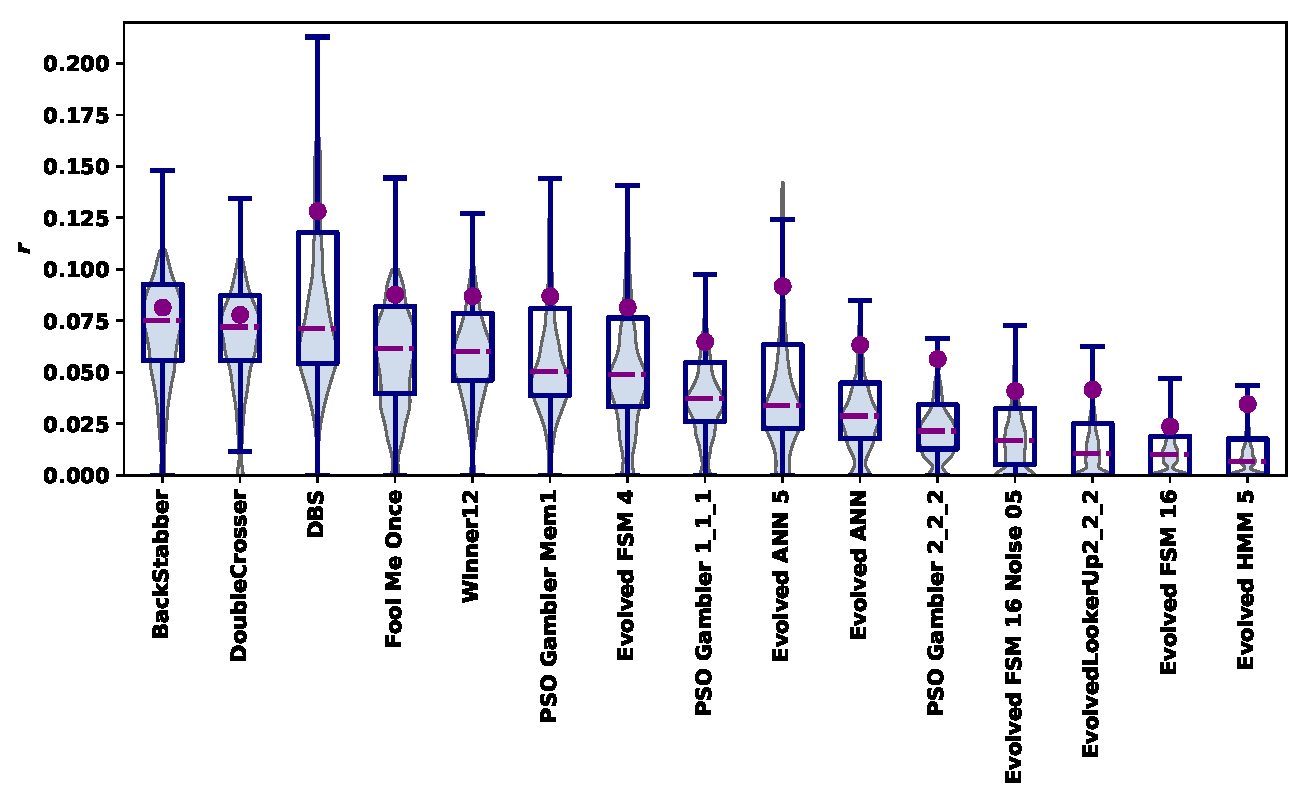
\includegraphics[width=\textwidth]{../images/performance_standard.pdf}
    \caption{P.D.}\label{fig:std_results}
\end{figure}


\newpage
\subsubsection{Noisy Tournaments}

The noisy tournament top 14 performances, based on \(\bar{R}\) are given
by Table~\ref{table:noisy_results}. The distributions of their \(R\) is also
given by Figure~\ref{fig:std_results}.


\begin{table}
    \begin{center}
    \begin{tabular}{lr}
\toprule
Name                &                        $\bar{r}$\\
\midrule
Grumpy              &                         0.13953 \\
$e$                 &                         0.19048 \\
Cooperator          &                         0.19565 \\
Tit For 2 Tats      &                         0.20520 \\
Cycle Hunter        &                         0.22222 \\
Risky QLearner      &                         0.22424 \\
Retaliate 3         &                         0.23077 \\
Retaliate 2         &                         0.23762 \\
Retaliate           &                         0.24309 \\
Hard Tit For 2 Tats &                         0.24658 \\
Limited Retaliate 3 &                         0.25000 \\
ShortMem            &                         0.25272 \\
Limited Retaliate   &                         0.25698 \\
Limited Retaliate 2 &                         0.26027 \\
$\phi $              &                         0.26201 \\
\bottomrule
\end{tabular}

    \caption{Noisy top performances}\label{table:noisy_results}
    \end{center}
\end{table}

\begin{figure}
    \centering
    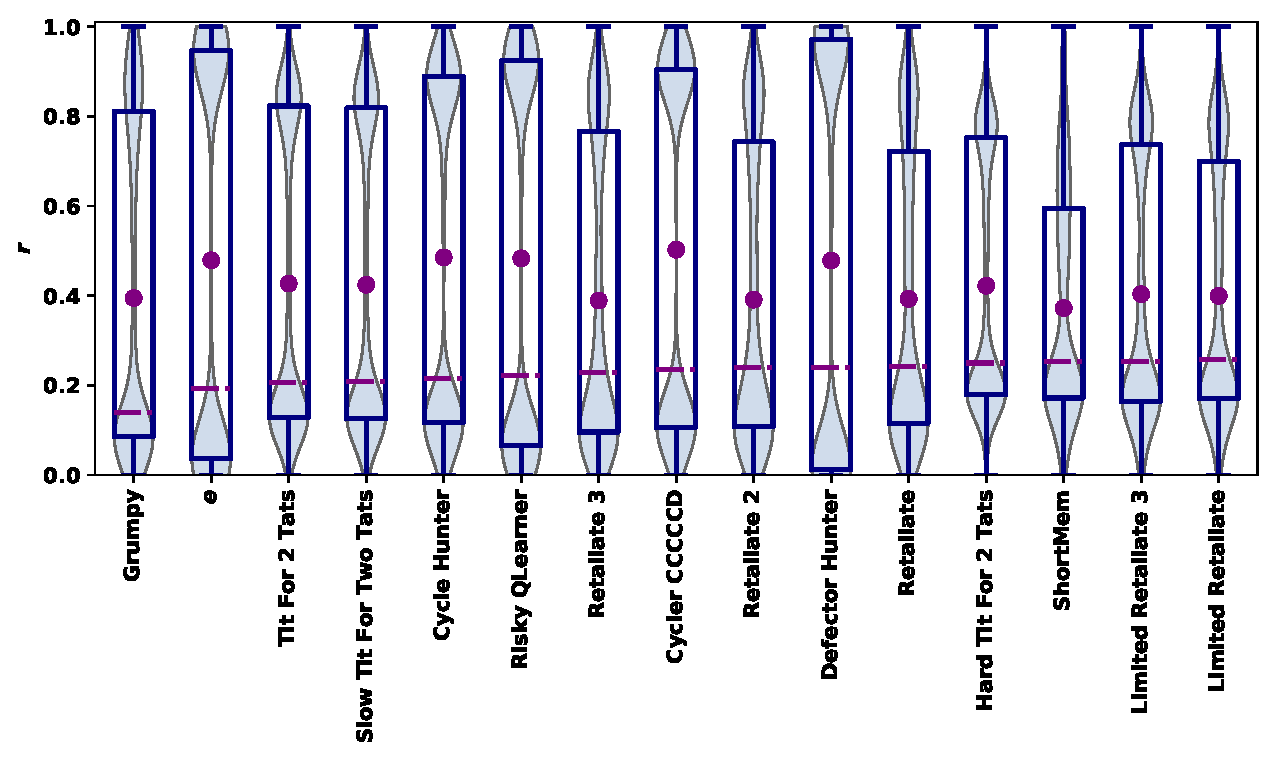
\includegraphics[width=.9\textwidth]{../images/performance_noise.pdf}
    \caption{\(R\) distributions for best performed strategies in noisy tournaments.}
\end{figure}

\subsubsection{Probabilistic ending Tournaments}

\begin{table}
    \begin{center}
    \begin{tabular}{lr}
\toprule
Name              &        $\bar{r}$                 \\
\midrule
Fortress4         &                           0.01266 \\
Defector          &                           0.01444 \\
Better and Better &                           0.01587 \\
Tricky Defector   &                           0.01869 \\
Fortress3         &                           0.02198 \\
Gradual Killer    &                           0.02521 \\
Aggravater        &                           0.02797 \\
Raider            &                           0.03077 \\
Cycler DDC        &                           0.04545 \\
Hard Prober       &                           0.05085 \\
SolutionB1        &                           0.06040 \\
Meta Minority     &                           0.06040 \\
Bully             &                           0.06061 \\
Fool Me Forever   &                           0.07018 \\
EasyGo            &                           0.07065 \\
\bottomrule
\end{tabular}

    \end{center}
\end{table}

\begin{figure}
    \centering
    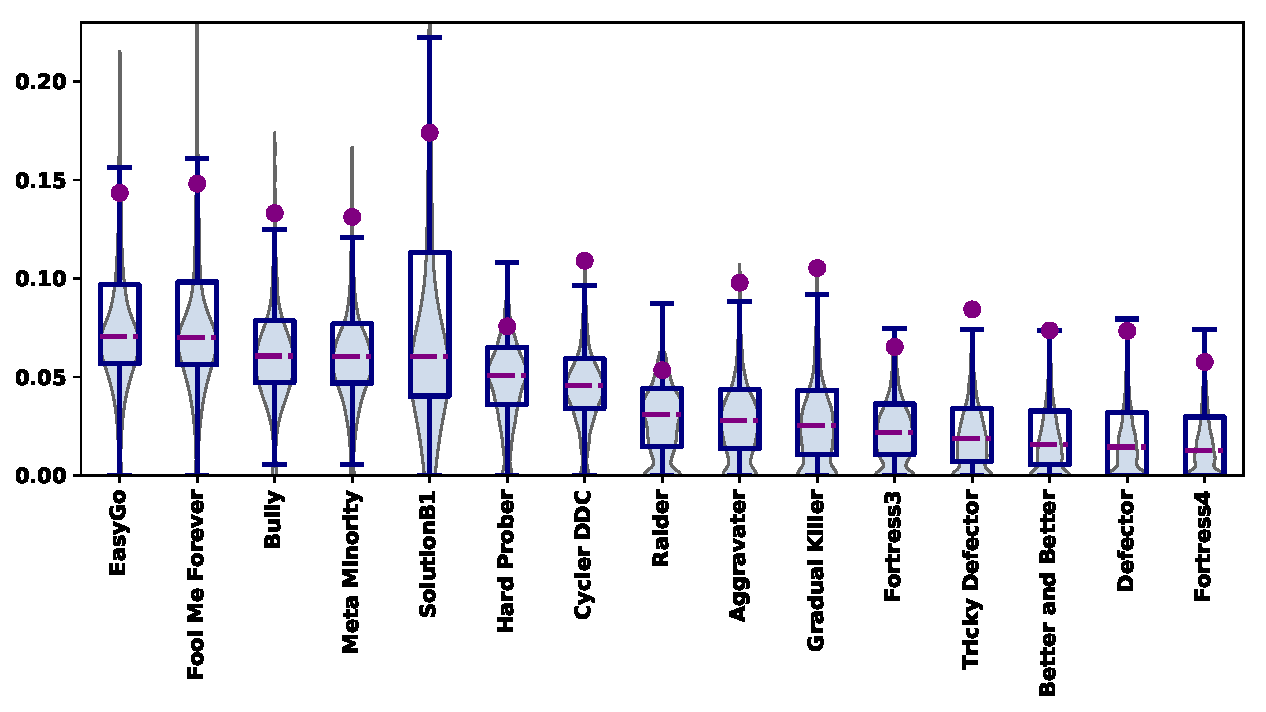
\includegraphics[width=.9\textwidth]{../images/performance_probend.pdf}
\end{figure}

\subsubsection{Noisy \& Probabilistic ending Tournaments}

\begin{table}
    \begin{center}
    \begin{tabular}{lr}
\toprule
Name                &                         $\bar{r}$    \\
\midrule
Alternator          &                                 0.30390 \\
$\phi$              &                                 0.31025 \\
$e$                 &                                 0.31293 \\
$\pi$               &                                 0.31818 \\
Limited Retaliate   &                                 0.35294 \\
Anti Tit For Tat    &                                 0.35429 \\
Retaliate 3         &                                 0.35484 \\
Limited Retaliate 3 &                                 0.35563 \\
Retaliate           &                                 0.35588 \\
Retaliate 2         &                                 0.35714 \\
Limited Retaliate 2 &                                 0.36066 \\
Hopeless            &                                 0.36913 \\
Arrogant QLearner   &                                 0.40526 \\
Cautious QLearner   &                                 0.40711 \\
Risky QLearner      &                                 0.41989 \\
\bottomrule
\end{tabular}

    \end{center}
\end{table}

\begin{figure}
    \centering
    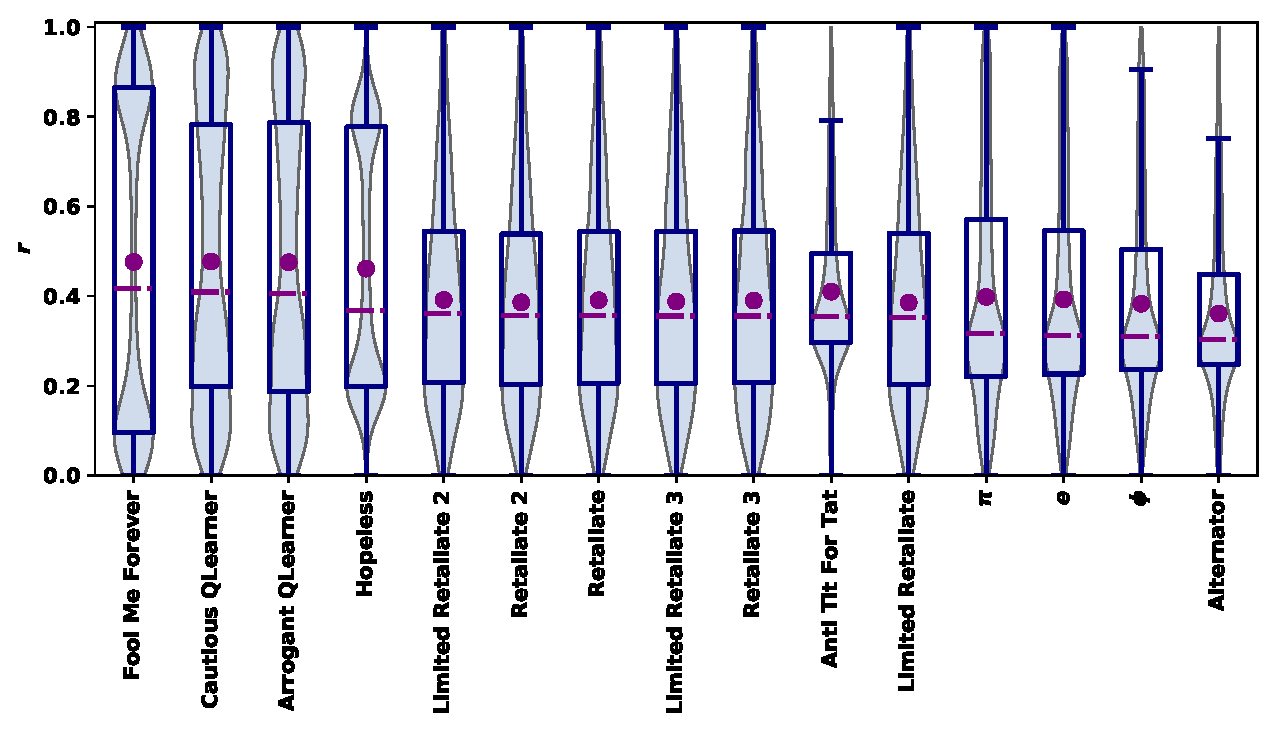
\includegraphics[width=.9\textwidth]{../images/performance_probend_noise.pdf}
\end{figure}

\subsubsection{Overall Tournaments}

\begin{table}
    \begin{center}
    \begin{tabular}{lr}
\toprule
{} &  Normalized\_Rank \\
Name                    &                  \\
\midrule
Evolved FSM 16          &            0.018 \\
Evolved HMM 5           &            0.019 \\
Evolved FSM 16 Noise 05 &            0.025 \\
EvolvedLookerUp2\_2\_2    &            0.028 \\
Evolved ANN             &            0.037 \\
PSO Gambler 2\_2\_2       &            0.040 \\
Evolved ANN 5           &            0.046 \\
PSO Gambler 1\_1\_1       &            0.061 \\
Fool Me Once            &            0.067 \\
Evolved FSM 4           &            0.075 \\
DoubleCrosser           &            0.079 \\
Winner12                &            0.081 \\
BackStabber             &            0.082 \\
DBS                     &            0.086 \\
PSO Gambler Mem1        &            0.089 \\
\bottomrule
\end{tabular}

    \end{center}
\end{table}


\begin{figure}
    \centering
    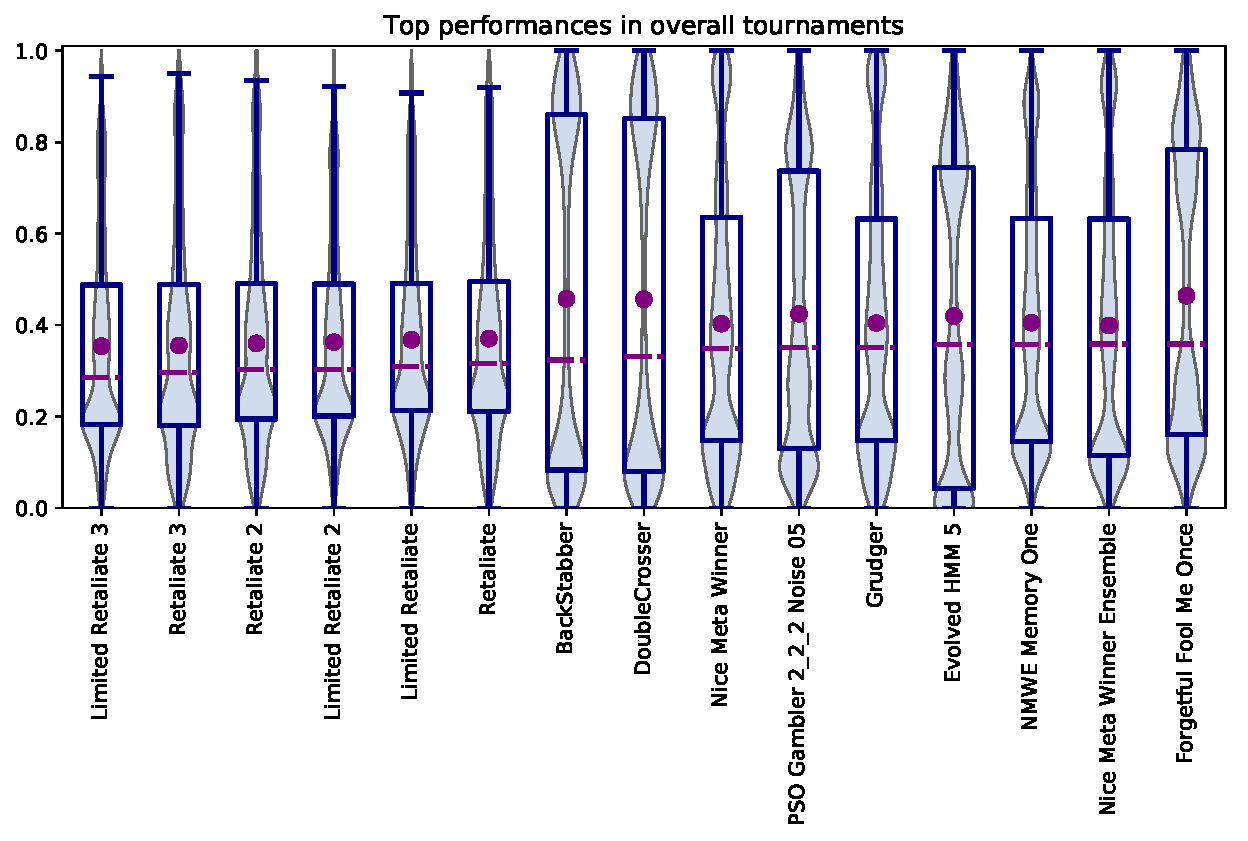
\includegraphics[width=.9\textwidth]{../images/performance_merged.pdf}
\end{figure}


\section{Evaluation of performance}\label{section:evaluation_of_performance}

\begin{figure}
    \centering
    \includegraphics[width=.7\textwidth]{../output/output/standard/feature_importance_bar_plot.pdf}
\end{figure}

\section{Conclusion and Discussion}\label{section:conclusion}

\bibliographystyle{plain}
\bibliography{bibliography}
\end{document}